%-------------------------------------------------
%
% Time.tex
%
%------------------------------------------------
\section[Tempi di risoluzione]{tempi di risoluzione}
\label{pt1:time}
Al fine di stabilire fino a quale dimensione il problema possa essere risolto in tempi, ragionevolmente brevi, ed in modo esatto si è deciso di valutare l'algoritmo sulle seguenti proprietà che contraddistinguono le istanze:

\begin{itemize}
\item numero di nodi del grafo;
\item distribuzione dei nodi sulla superficie della piastra.
\end{itemize}

Inizialmente si è proceduto, nel seguente modo, alla generazione delle istanze; si sono create delle classi di istanze e per ognuna di esse si sono create 5 istanze differenti ma che condividessero le proprietà sopra riportate.

Successivamente si è eseguito l'algoritmo su ciascuna di esse e si sono registrati, nel foglio di calcolo allegato, i vari tempi di esecuzione ed il valore della funzione obiettivo.

\begin{table}[htbp]
\centering
\label{pt1:time:tabular}
\begin{tabular}{|c|c|c|c|}
\hline
\textbf{Classe} & \textbf{AVG Random (ms)} & \textbf{AVG Cluster (ms)} & \textbf{AVG Circle (ms)}\\
\hline
5   &     19 &     18 &   13 \\
\hline
10  &     73 &     88 &   38 \\
\hline
15  &    238 &    192 &   50 \\
\hline
20  &    397 &    381 &   67 \\
\hline
30  &   1872 &  12685 &  113 \\
\hline
40  &   6054 &  33123 &  275 \\
\hline
50  &  13308 &   7834 & 2754 \\
\hline
60  &  20883 &  35698 & 3587 \\
\hline
70  &  40550 &  63743 &  766 \\
\hline
80  &  92111 & 292809 & 3121 \\
\hline
90  & 256191 & 197488 & 2415 \\
\hline
100 & 506619 & 823554 & 5242 \\
\hline
\end{tabular}
\caption{Tempi medi di esecuzione}
\end{table}

Nella Tabella \ref{pt1:time:tabular} sono riportate le medie dei tempi riscontrati.

\begin{figure}
\centering
\begin{subfigure}[b]{0.9\textwidth}
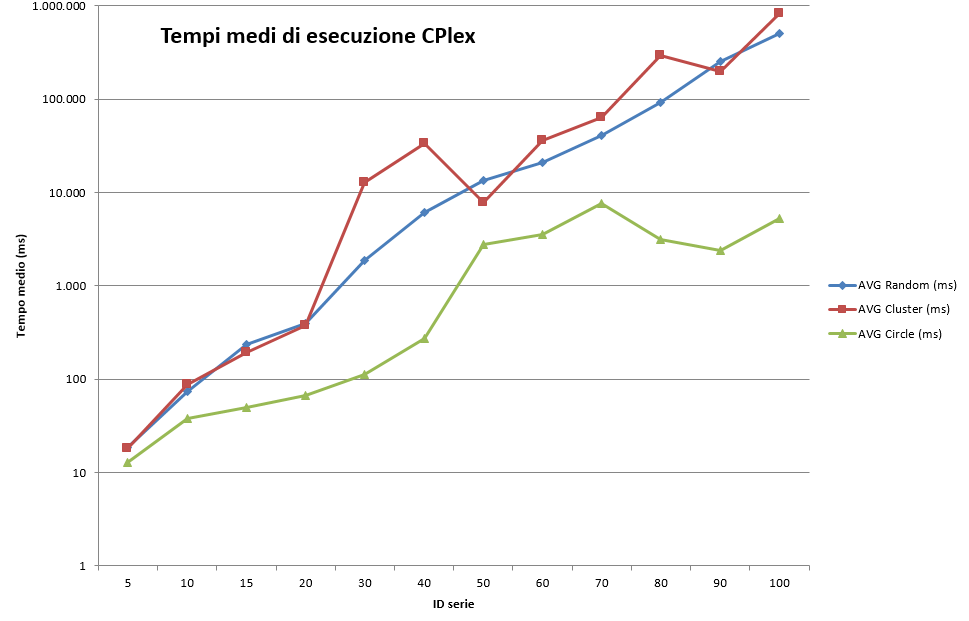
\includegraphics[width=\textwidth]{Images/Part_1/graphics/Times01.png}
\caption{Tempi di risoluzione al variare dei punti}
\label{pt1:time:time01}
\end{subfigure}

\begin{subfigure}[b]{0.9\textwidth}
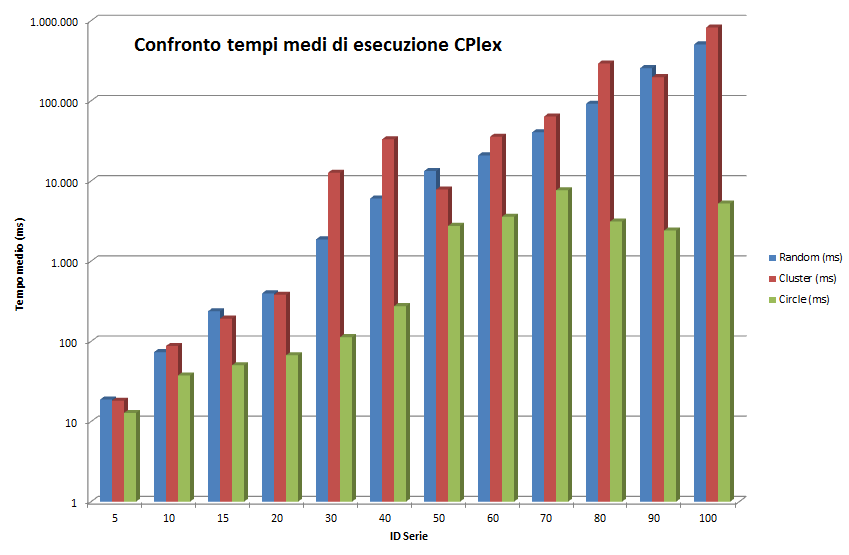
\includegraphics[width=\textwidth]{Images/Part_1/graphics/Times02.png}
\caption{Tempi di esecuzione per tipologia}
\label{pt1:time:time02}
\end{subfigure}
\caption{Confronto tempistiche}
\label{pt1:time:times}
\end{figure}

\subsection[Conclusioni]{conclusioni}
\label{pt1:time:conclusion}
Dalle misurazioni effettuate si evince che all'aumentare dei punti che compongono l'istanza vi è un significativo aumento nei tempi di risoluzione, in modo esatto del modello.

Più precisamente, come si può notare in figura \ref{pt1:time:time01} (N.B. scala dei tempi logaritmica), il tempo di risoluzione del problema cresce esponenzialmente all'aumentare dei nodi che compongono il grafo.

Essendo il TSP un problema \english{NP-hard}, la sua risoluzione richiede degli algoritmi a complessità esponenziale perciò i risultati ottenuti sono coerenti con quanto atteso.